\chapter{Individual Cetacean ID via Automatic Most Likely Catalogue Matching}\label{ch:ID}

This Chapter examines the final component in the automatic photo-id pipeline, focussing on individual identification. The component takes as input photo-id catalogue images which have been passed through the dorsal fin detector and post-processing methodology outlined in Chapter \ref{ch:cetDet} to produce a list of most likely catalogue matches. It is important to note here that this component does not intend to replace photo-id researchers by performing the job for them. Instead, the component aims to vastly reduce the search space the researcher needs to examine in order to verify a catalogue match; the component suggests a list of most likely catalogue matches, but ultimately the final decision lies with the researcher.

Beginning by outlining the requirements an automatic system for most likely catalogue matching must meet, the Chapter then discusses possible approaches to the problem and justification for the selected approach. System development is discussed in detail, using the NDD AU SMRU dataset created in Chapter \ref{ch:NDD} for training and evaluation. Discussion of further processing techniques and their effect on most likely catalogue matching accuracy is discussed, alongside the current limitations of the approach. 

\section{Most Likely Catalogue Matching System Requirements}\label{ch:ID,sec:Requirements}

Before development can begin it is important to outline the requirements of a system capable of most likely catalogue matching. Unlike the detector which could be considered a coarse-grain task, identification of individual cetaceans is an extremely fine-grain problem as they are distinguished from each other using small prominent markings present on the dorsal fin. As the animals are free roaming, there can be high variation in how the fin is captured in the image, discussed in greater detail in Section \ref{ch:cetDet,sec:requirements,sub:environmental}. This can lead to photo-id catalogues with low inter-class but high intra-class differences between the individuals present, seen in Figure \ref{fig:segmented-ndd20-example}. As a result of this, any system capable of accurate catalogue matching must be able to recognise these minute differences between individuals even when there is high variation in the examples for each individual class. 

The system must also be capable of operating using all information provided to it. Other photo-id aides which perform most likely catalogue matching such as finFindR \cite{thompson_finfindr_2022} operate using only the trailing edge of the fin, with matching performed using notches and shape. This misses other prominent markings such as long term scarring or pigmentation, as well as the shape of other fin edges. As such, it may be the case that finFindR struggles when operating over a catalogue with few to no notches. To avoid this issue, the system developed must be capable of matching using all available prominent markings. 

Further, the system must also be capable of performing accurate catalogue matching under the presence of noise, both classified and misclassified. Datasets developed for the training of this system such as NDD AU SMRU contain a \texttt{noise} class which encapsulates all detected mask components which are erroneously retained after post-processing has been applied. This class has extremely high intra-class variance, however it is imperative the system is able to match erroneous components to it. Misclassified noise is defined as that which has been passed downstream as a result of being attached to a valid individual detection mask. In Figure \ref{fig:crop-with-unclassified-noise} for example, the swell captured in the post-processed crop would be considered misclassified noise. Any system performing automatic most likely catalogue matching must be resistant to small amounts of misclassified noise in order to produce accurate identity suggestions.

\begin{figure}
	\begin{center}
		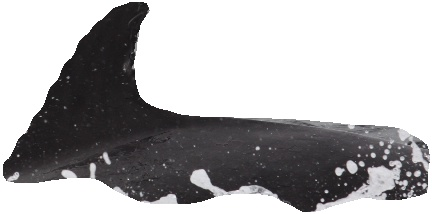
\includegraphics[scale=0.6]{Chapter5/figs/crop-with-unclassified-noise.jpg}
	\end{center}
	\caption{An example post-processed crop which contains some misclassified noise.}
	\label{fig:crop-with-unclassified-noise}
\end{figure}

Any developed system must also be capable of handling examples of individuals which are not present in the photo-id catalogue. Due to the free roaming nature of cetaceans (or indeed any wild animal) and the limitations on photo-id survey size dictated by both weather and workforce, there is no guarantee that every animal who makes use of the survey area will be captured. New animals may also become resident in the area through birth or migration. When these animals are eventually captured during a survey and their image processed, the system must be capable of recognising this as an individual not currently present in the catalogue and highlight this to the researcher. This is made more difficult given the extreme fine-grain nature of the catalogues. As a result, this requirement necessitates the system must be capable of recognising uncertainty or understand a notion of similarity between an input and the class examples present in the catalogue. 

In traditional computer vision classification models, if a new class were to be added this would require a large number of example images of the new class as well as model retraining or fine-tuning. However, cetacean researchers are highly unlikely to possess the technical skills required to retrain or fine-tune a computer vision model, and even if they do it is unlikely a large number of example images for the new individual would be available to do so. As such, the system must be adaptable enough so as to not require extensive retraining when new individuals are added to the catalogue.

\section{Deciding on Approach}\label{ch:ID,sec:deciding}

Out of all requirements an automatic most likely catalogue matching system must meet, arguably the most important is the need for flagging of previously unseen individuals. As noted, this necessitates any underlying computer vision model to have some notion of uncertainty or similarity. It is this requirement that guided approach selection. 

\subsection{Bayesian Dropout}\label{ch:ID,sec:deciding,sub:bayesianDropout}

Traditional computer vision classification models do not meet this requirement. If an example image of a new individual was seen by a traditional CNN trained on a photo-id catalogue dataset, this model would still attempt to provide a classification based on the classes present at train time.  As deep computer vision models operate on point estimations of parameters, unlike Gaussian processes where the probability distribution is defined over a function, this removes the ability to produce helpful indicators of uncertainty such as prediction confidence bounds \cite{gal_uncertainty_2016}. 

One way to create a notion of uncertainty from this is through the use of Bayesian dropout. Vanilla dropout has found widespread use in the training of generalisable deep learning models. At train time, nodes in the model are intentionally not updated during a training step with some probability, usually defined as a hyperparameter with the goal of aiding model generalisability \cite{srivastava_dropout:_2014}. At test time, no dropout is performed and all nodes are utilised for the prediction. 

Bayesian dropout re-frames this technique by also performing dropout at test time, again with some hyperparameter defined probability \cite{gal_dropout_2016}. For each classification output, the model performs inference some large $N$ number of times. During each run model nodes are randomly disabled, zeroing out their weight and effecting the ability of the model to produce a prediction. By performing this multiple times and producing $N$ classifications, a probabilistic distribution is determined which can be used to understand the uncertainty of the model. A final overall prediction is generated by taking the mean of all $N$ predictions used to generate the probability distribution. If randomly dropping nodes at test time results in the model producing a wide variety of outputs, resulting in a diffused probability distribution, this suggests the model is uncertain; the lower the variance of the probability distribution, the more certain the model is. 

Whilst Bayesian dropout has found use in areas such as time-series forecasting \cite{laptev_time-series_2017}, widespread use has not been adopted in areas such as computer vision despite attempts \cite{kendall_what_2017}. This can be contributed to recognised issues such as ill-defined variational objective, the use of improper priors, and the potential for clarity issues between model uncertainty and risk \cite{hron_variational_2018, osband_risk_2016}. Further to this, the computational expense of performing Bayesian dropout is large given the need for multiple inferences required to produce the classification probability distribution.

This is the main reason why Bayesian dropout was not utilised for automated most likely catalogue matching. Should a researcher wish to process a large batch of images after a field survey for example, the need for multiple inferences would vastly inflate the time required for the batch operation to complete. Issues also arise meeting other system requirements. Even when using Bayesian dropout, the underlying model would still require retraining or fine-tuning to output newly catalogued individuals. 

\subsection{Siamese Neural Networks}\label{ch:ID,sec:deciding,sub:SNN}

Rather than producing a classification and measuring uncertainty as is the case with Bayesian dropout, Siamese Neural Networks (SNNs) aim to incorporate the notion of similarity in the model. SNNs are made up of at least two parallel identical CNNs; they share the same backbone architecture, initial and updated weights, and hyperparameters. This consistency allows the SNN to compare the inputs received by each CNN branch, producing a similarity score between the outputs rather than a direct classification. A visualisation of a two branch SNN can be seen in Figure \ref{fig:signet-SNN-architecture}.

\begin{figure}
	\begin{center}
		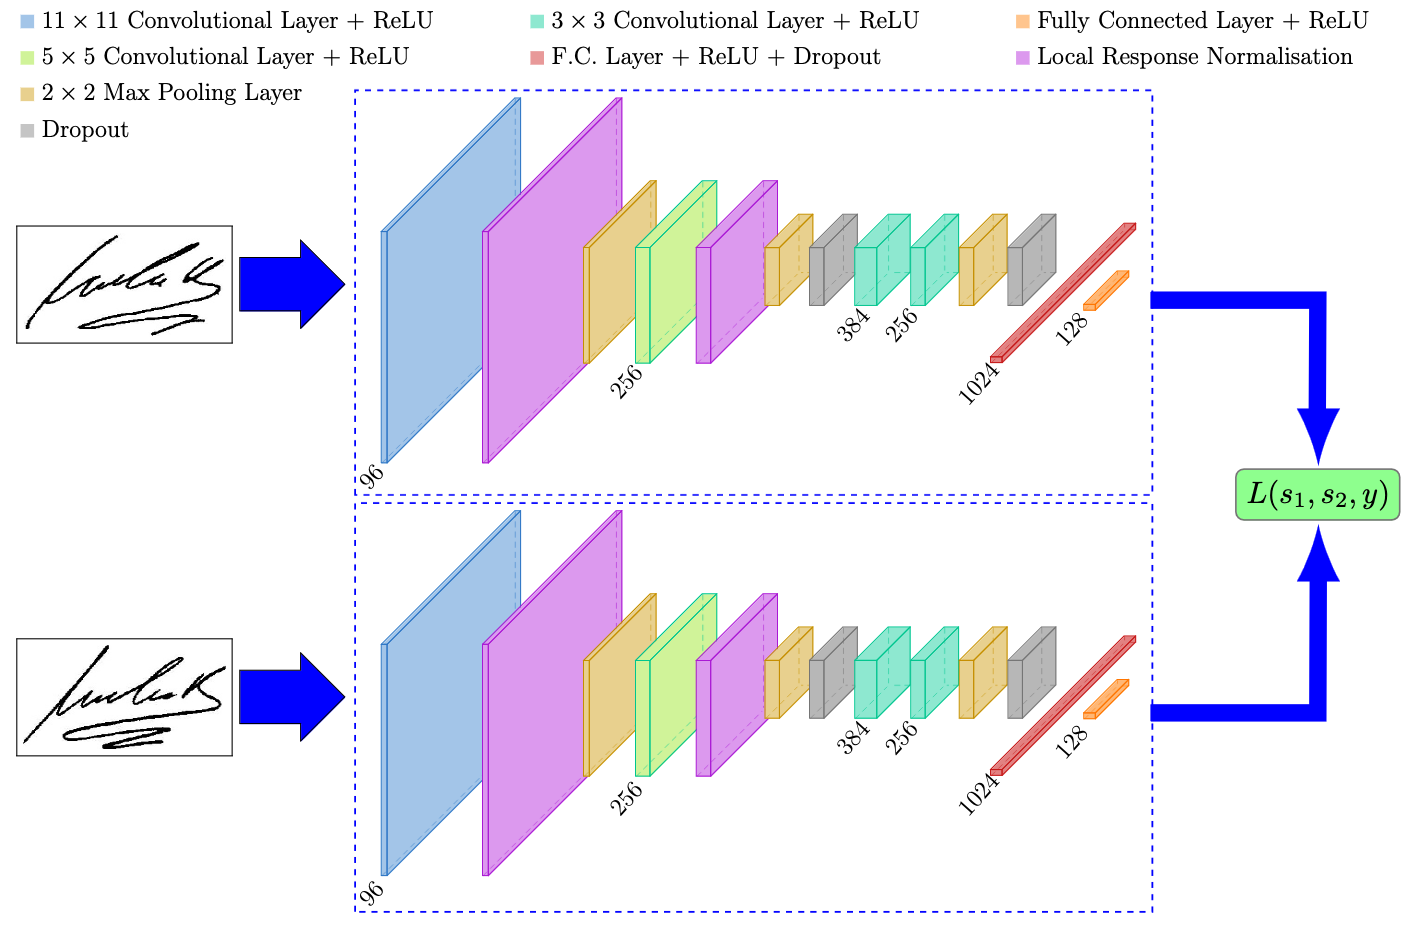
\includegraphics[scale=0.4]{Chapter5/figs/signet-SNN-architecture.png}
	\end{center}
	\caption{A visualisation of an example SNN architecture. Image from \cite{dey_signet_2017}.}
	\label{fig:signet-SNN-architecture}
\end{figure}

Each parallel CNN which forms an SNN branch is designed to produce an embedding, or a lower dimensional representation, of the input it receives through the use of an embedding layer placed at the end of the CNNs architecture. It is these generated embeddings which are utilised to optimise the loss function, rather than the model inputs themselves. As common CNN architectures often make use of an embedding layer before their final softmax layer, it is routine to see SNNs created simply by removing the softmax layer of a common CNN architecture and parallelising. Thanks to this ability to perform similarity comparison SNNs have been utilised for multiple problems in computer vision, for example in signature verification \cite{dey_signet_2017} or vehicle re-identification \cite{wang_discriminative_2020}. Specifically in conservation tech, SNNs have found use in fine-grain species identification problems \cite{vetrova_hidden_2018, araujo_two-view_2022} as well as in more extreme fine-grain individual animal identification \cite{clapham_automated_2020}. 


% Follow Format of https://towardsdatascience.com/how-to-train-your-siamese-neural-network-4c6da3259463
% Rework description of embedding above to include example like in ^ ?
% Discuss how the embedding generated is used for similarity. Train time needing all branches and test time only using one. Generated embedding plotted into N-dimensional latent space. Euclidean distance used for distance measurement. etc.

% Introduce triplet loss. Semi-Hard triplet mining. Prototypes.






%%%%%%%%%%%%%%%%%%%
